%%****************************************************************************
%** Copyright 2002, 2003 by Lukas Ruf, <ruf@topsy.net>
%** Information is provided under the terms of the
%** GNU Free Documentation License <http://www.gnu.org/copyleft/fdl.html>
%** Fairness: Cite the source of information, visit <http://www.topsy.net>
%****************************************************************************
%** Last Modification: 2013-07-31
%** 2005-07-11	Bernhard Tellenbach
%**							Switched default document class to: book
%**							Added %%****************************************************************************
%** Copyright 2005 by Bernhard Tellenbach, <bernhard.tellenbach@airmail.ch>
%** Information is provided under the terms of the
%** GNU Free Documentation License <http://www.gnu.org/copyleft/fdl.html>
%****************************************************************************
%****************************************************************************
%** Last Modification: 2005-07-11 1600
%** 2005-07-11	Updated the syntax to match the current nomencl packet
%****************************************************************************

\chapter{\label{appendixA}Title}


\section{\label{chapterA:section1}Section 1}

\begin{verbatim}
All is presented exactely the way you write it.

Page boundaries are not checked.....................................................................................

\end{verbatim}

\chapter{\label{appendixB}Title}


%Entries for the list of abbrevations:
%
%To generate the list of abbrevations, execute:
%makeindex Thesis.nlo -s nomencl.ist -o Thesis.nls
%
%If you are using TeXniCenter, specify:
%"%bm.nlo" -s nomencl.ist -o "%bm.nls"
%as beeing the argument list for makeindex.
%---------------------------------------------------------------------------------------------------------
%For old nomencl package uncomment this:
%\printglossary
%For new nomencl package uncomment this:
\printnomenclature

\abbrev{XCA}{\markup{X}tremely \markup{C}ool \markup{A}bbrevations}



%** 2013-07-31 David Gugelmann (gugdavid)
%**            Use bibtex for references
%**            Added new watermark command
%****************************************************************************



\documentclass[10pt,final,a4paper,twoside]{book}
%\documentclass[10pt,draft,a4paper,oneside]{report}
%\documentclass[10pt,draft,a4paper,oneside]{article}

%**Latex Master Document*********

%** preamble.tex: here all the document-wide settings
%                 are defined
%****************************************************************************
%** Copyright 2001, 2002, 2003, 2004 by Lukas Ruf, <lukas.ruf@lpr.ch>
%** Information is provided under the terms of the
%** GNU Free Documentation License <http://www.gnu.org/copyleft/fdl.html>
%** Fairness: Cite the source of information, visit <http://www.topsy.net>
%****************************************************************************
%** Last Modification: 2013-07-31
%** 2004-02-17: Lukas Ruf
%**             Added recommendation by Thomas Duebendorfer
%**             Added different babel languages
%**             Added more comments
%** 2004-10-16: Lukas Ruf
%**             More comments
%**             Added subfigure
%** 2005-07-11	Bernhard Tellenbach
%**							Added \abbrev command to generate a list of abbrevations
%**							Removed support for psfig and epsfig (old)
%** 						Adapted syntax for new nomencl packet version
%** 2013-07-31 David Gugelmann (gugdavid)
%**            Adapted for pdflatex
%**            Added hyperref
%**            Style of headers modified, adapted watermark command
%****************************************************************************

\RequirePackage{times}

\usepackage[english]{babel}
%-% \usepackage[german]{babel}
%-% \usepackage[ngerman]{babel}

\usepackage[utf8]{inputenc}
\usepackage[T1]{fontenc}
\usepackage{type1cm}

\usepackage{a4}

\usepackage{hyperref}
\hypersetup{colorlinks,%
            citecolor=black,%
            filecolor=black,%
            linkcolor=black,%
            urlcolor=black,%
            pdftex}

\usepackage[pdftex]{color,graphicx} % pdftex does not read eps files -> use epstopdf to convert files
\graphicspath{{Figures/},{logos/}}

\usepackage{caption}
\usepackage{subcaption} % caption/subcaption replaces subfigure, which is deprecated

\usepackage{fancyhdr}
\usepackage{fancybox}

\usepackage{float}
\usepackage{longtable}
\usepackage{paralist}
\usepackage{url}
\usepackage{lscape}
\usepackage{moreverb}
\usepackage{pdfpages}

\usepackage{nomencl}
  \let\abbrev\nomenclature
  \renewcommand{\nomname}{List of Abbrevations}
  \setlength{\nomlabelwidth}{.25\hsize}
  \renewcommand{\nomlabel}[1]{#1 \dotfill}
  \setlength{\nomitemsep}{-\parsep}
  %For old nomencl package, uncomment this:
  \makeglossary 
  %For new nomencl package, uncomment this:
  %\makenomenclature

\usepackage[normalem]{ulem}
  \newcommand{\markup}[1]{\uline{#1}}
  
%% Thanks to Thomas Duebendorfer: Should create smoother fonts
\usepackage{ae,aecompl}

\addtolength{\textwidth}{2cm}
\addtolength{\textheight}{2cm}
\addtolength{\oddsidemargin}{-1.0cm}
\addtolength{\evensidemargin}{-1.0cm}
\addtolength{\topmargin}{-1.5cm}

%% No Serifs: Put comment markers in front of the next three lines otherwise
\renewcommand{\ttdefault}{cmtt}
\renewcommand{\rmdefault}{phv}  % Helvetica for roman type as well as sf
\renewcommand{\ttdefault}{pcr}  % use Courier for fixed pitch, if needed

\newcommand{\?}{\discretionary{/}{}{/}}
\newcommand{\liter}[0]{/home/ruf/Lib/Bibl/}
\newcommand{\fref}[1]{\mbox{Figur~\ref{#1}}}

\pagestyle{fancy}
%%-lpr Note: 'chapters' are defined for 'book's only
%%-lpr       in articles, we make use of sections only
%%-lpr \renewcommand{\chaptermark}[1]{\markboth{#1}{}}
\renewcommand{\sectionmark}[1]{\markright{\thesection\ #1}}
\fancyhf{}
\fancyhead[LE,RO]{\bfseries\thepage}
\fancyhead[LO]{\bfseries\rightmark}
\fancyhead[RE]{\bfseries\leftmark}
\renewcommand{\headrulewidth}{0.5pt}
\addtolength{\headheight}{0.5pt}
\fancypagestyle{plain}{%
   \fancyhf{}
   \fancyfoot[C]{\bfseries \thepage}
   \fancyhead{}%get rid of headers on plain pages
   \renewcommand{\headrulewidth}{0pt} % an the line
}
\newcommand{\clearemptydoublepage}{\newpage{\pagestyle{empty}\cleardoublepage}}

\setlength{\parindent}{0in}

\hyphenation{Lukas not-to-hyphen-else-where}

\newcommand{\Appendix}[2][?]
{
  \refstepcounter{section}
  \addcontentsline{toc}{appendix}
  {
    \protect\numberline{\appendixname~\thesection} %1
  }
  {
    \flushright\large\bfseries\appendixname\ \thesection\par
    \nohypens\centering#1\par
  }
  \vspace{\baselineskip}
}

\let\margin\marginpar
\newcommand\myMargin[1]{\margin{\raggedright\scriptsize #1}}
\renewcommand{\marginpar}[1]{\myMargin{#1}}

\newcommand\CHECK{\myMargin{CHECK}}
\newcommand\NEW{\myMargin{NEW}}

%% adapt headers %%
% from http://www.markschenk.com/tensegrity/latexexplanation.html
% Result:
% - No headers on empty pages before new chapter
% - To avoid header on other pages (e.g. in the abstract), set pagestlye to plain
\makeatletter
\def\cleardoublepage{\clearpage\if@twoside \ifodd\c@page\else
    \hbox{}
    \thispagestyle{plain}
    \newpage
    \if@twocolumn\hbox{}\newpage\fi\fi\fi}
\makeatother

%% allow to set a watermark %%
% from http://www.goodcomputingtips.com/site/2010/06/how-to-insert-watermark-in-latexpdflatex-documents/
% - to include a watermark, define \watermark in the main document, e.g.: \newcommand{\watermark}{MY WATERMARK TXT}
\ifdefined\watermark
  \usepackage{graphicx,type1cm,eso-pic,color}
  \makeatletter
            \AddToShipoutPicture{
              \setlength{\@tempdimb}{.5\paperwidth}
              \setlength{\@tempdimc}{.5\paperheight}
              \setlength{\unitlength}{1pt}
              \put(\strip@pt\@tempdimb,\strip@pt\@tempdimc){
          \makebox(0,0){\rotatebox{55}{\textcolor[gray]{0.95}
          {\fontsize{5cm}{5cm}\selectfont{\watermark}}}}
              }
          }
  \makeatother
\fi


%********************************

%** begin the document environment
\begin{document}

\frenchspacing
\sloppy

%** Title.tex: Title page to be printed first
  %****************************************************************************
  %** Copyright 2002 by Lukas Ruf, ruf@topsy.net
  %** Information is provided under the terms of the
  %** GNU Free Documentation License http://www.gnu.org/copyleft/fdl.html
  %** Fairness: Cite the source of information, visit http://www.topsy.net
  %****************************************************************************
  %** Extensions:
  %** January 2003: Thomas Duebendorfer <thomas@duebendorfer.ch>
  %**   changed the former ETH Header to the new, official one that is
  %**   mandatory since January 2003.
  %****************************************************************************
  %****************************************************************************
  %** Extensions:
  %** January 2005: Bernhard Tellenbach <bernhard.tellenbach@airmail.ch>
  %**   changed the way the ETH Header is included. Slight modification of the
  %**   content.
  %****************************************************************************
  \begin{titlepage}

  \begin{center}
  \begin{figure}[!t]
     
\includegraphics{TIKETHhdr}
  \end{figure}
  \end{center}

  \vspace{2 cm}

  {\large Philipp Mao}
  \vspace{2 cm}

  {\Huge Boosting the convergence \\ performance of SDX platforms}\\

  \vspace{\fill}


  Semester Thesis SA -2016-69\\
  October 2016 to January 2017\\

  \vspace{1cm}
  Tutor: Rüdiger Birkner \\
  Supervisor: Laurent Vanbever \\
    
  \end{titlepage}


%** environments.tex: Predefined Environments
%****************************************************************************
%** Copyright 2002 by Lukas Ruf, ruf@topsy.net
%** Information is provided under the terms of the
%** GNU Free Documentation License http://www.gnu.org/copyleft/fdl.html
%** Fairness: Cite the source of information, visit http://www.topsy.net
%****************************************************************************

\newenvironment{sourcecode}%
{\vspace{0.5 cm} \footnotesize \verbatim}%
{\endverbatim \normalsize \vspace{0.5 cm}}

\newenvironment{inputverb}[1]%
{\vspace{0.5 cm} \footnotesize \verbatiminput{#1}}%
{\normalsize \vspace{0.5 cm}}

\newenvironment{inputverb_nospace}[1]%
{\footnotesize \verbatiminput{#1}}%
{\normalsize}



%**Documentation****************

%** Abstract.tex: Contains a brief description
%                 of what the reader may expect
%****************************************************************************
%** Copyright 2002 by Lukas Ruf, ruf@topsy.net
%** Information is provided under the terms of the
%** GNU Free Documentation License http://www.gnu.org/copyleft/fdl.html
%** Fairness: Cite the source of information, visit http://www.topsy.net
%****************************************************************************
%** Last Modification: 2005-07-11 1600
%** 2005-07-11	Bernhard Tellenbach
%**							Inserted new content
%****************************************************************************
\clearpage
\null
\vfil % or it might be \null
\thispagestyle{plain}
\begin{center}\textbf{Abstract}\end{center}
Remote failures in the Internet can lead to minutes of connectivity loss due to the long convergence time of BGP.

Swift is a fast reroute framework designed to shorten the convergence time of a BGP speaking router. Swift predicts the cause of a failure and then reroutes traffic to unaffected peers.  

Routers connected to a industrial scale software defined Internet exchange point (iSDX), suffer like any other BGP speaking router from long convergence times upon remote failure. 

In this work we show that it is possible to integrate Swift with minor modifications into the iSDX. The convergence time of all the participants of the swifted iSDX is improved by up to a factor 60. But as both Swift and the iSDX use the destination MAC address to encode information, the amount of bits available to Swift and the iSDX is reduced. This impacts Swift's performance and the iSDX's ability to scale with a higher number of participants. The introduced overhead by Swift to process a single BGP update is minimal. 
\vfil
\clearpage 


%** Table of Contents
\tableofcontents

%** Table of Figures
\listoffigures

%** Table of Figures
\listoftables

%** Introduction.tex: Contains an introduction to
%                     the topic and motivates the work.
%                     State what the reader can find where.
%****************************************************************************
%** Copyright 2002 by Lukas Ruf, ruf@topsy.net
%** Information is provided under the terms of the
%** GNU Free Documentation License http://www.gnu.org/copyleft/fdl.html
%** Fairness: Cite the source of information, visit http://www.topsy.net
%****************************************************************************

%Example structure for an introduction
%****************************************************************************
%** Copyright 2002, 2003 by Lukas Ruf, <ruf@topsy.net>
%** Information is provided under the terms of the
%** GNU Free Documentation License <http://www.gnu.org/copyleft/fdl.html>
%** Fairness: Cite the source of information, visit <http://www.topsy.net>
%****************************************************************************

\chapter{\label{introduction}Introduction}
The border gateway protocol is the glue that holds today's internet together. It allow autonomous networks to exchange information about reachability of prefixes without revealing their own network infrastructure. \\
Remote disruptions in BGP can lead to convergence times of multiple minutes. This long convergence time is caused by the way BGP updates are propagated through the internet. The convergence time is lower bounded by the time it takes for all BGP withdrawal updates to be received. \\
Software defined networking allows network operators to have more control over the network routing. It is also a technology that can help solve some of the internet's problems including long BGP convergence times. \\
In this work I will try to improve the convergence time of the industrial scale internet exchange point (iSDX) using the Swift framework, both rely on SDN switches to enable their functionality. 




%** Problem.tex: Documentation in own words of the problem to
%                be addressed in this document:
%                What is the challenge, why is it useful what you
%                plan to do.
%****************************************************************************
%** Copyright 2002 by Lukas Ruf, ruf@topsy.net
%** Information is provided under the terms of the
%** GNU Free Documentation License http://www.gnu.org/copyleft/fdl.html
%** Fairness: Cite the source of information, visit http://www.topsy.net
%****************************************************************************
%****************************************************************************
%** Last Modification: 2005-07-11 1600
%** 2005-07-11	Bernhard Tellenbach
%**							This is an addapted version of the Introduction.tex file
%**							Added table example (footnotes,multicolumn)
%**							Examples for different text sizes
%**							Updated eps file inclusion example for use with graphicx pkt. 
%****************************************************************************

\chapter{\label{chapter2}Background}

\section{\label{chapter2:iSDX}iSDX}
The iSDX is a framework for deploying software defined networking at internet exchange points. \\
An internet exchange point is a physical location where multiple autonomous systems meet to exchange traffic and BGP routes. \\
Deploying the iSDX at an internet exchange point gives participants more control over routing decisions. This is done by giving participants the opportunity to define policies. These policies allow participants to influence traffic coming from and going in the internet exchange point without obscure BGP message manipulation. The iSDX uses an SDN switch connected to the iSDX and all the participants to implement the policies as flowrules.
\subsection{\label{chapter2:iSDX:policies}policies}
Policies match on a field of the packet header and then forward the packet to a participant.
\paragraph{\label{chapter2:iSDX:policies:outbound policies}outbound policies:}
Outbound policies let participants direct packets going from themselves to the iSDX. They allow the participants to choose the participant the packet gets sent to.
\paragraph{\label{chapter2:iSDX:policies:inbound policies}inbound policies:}
Inbound policies allow participants to direct packets coming from the iSDX. In effect they allow the participant to choose to which of his own routers packets from the iSDX get sent to. 

\begin{figure}[h]
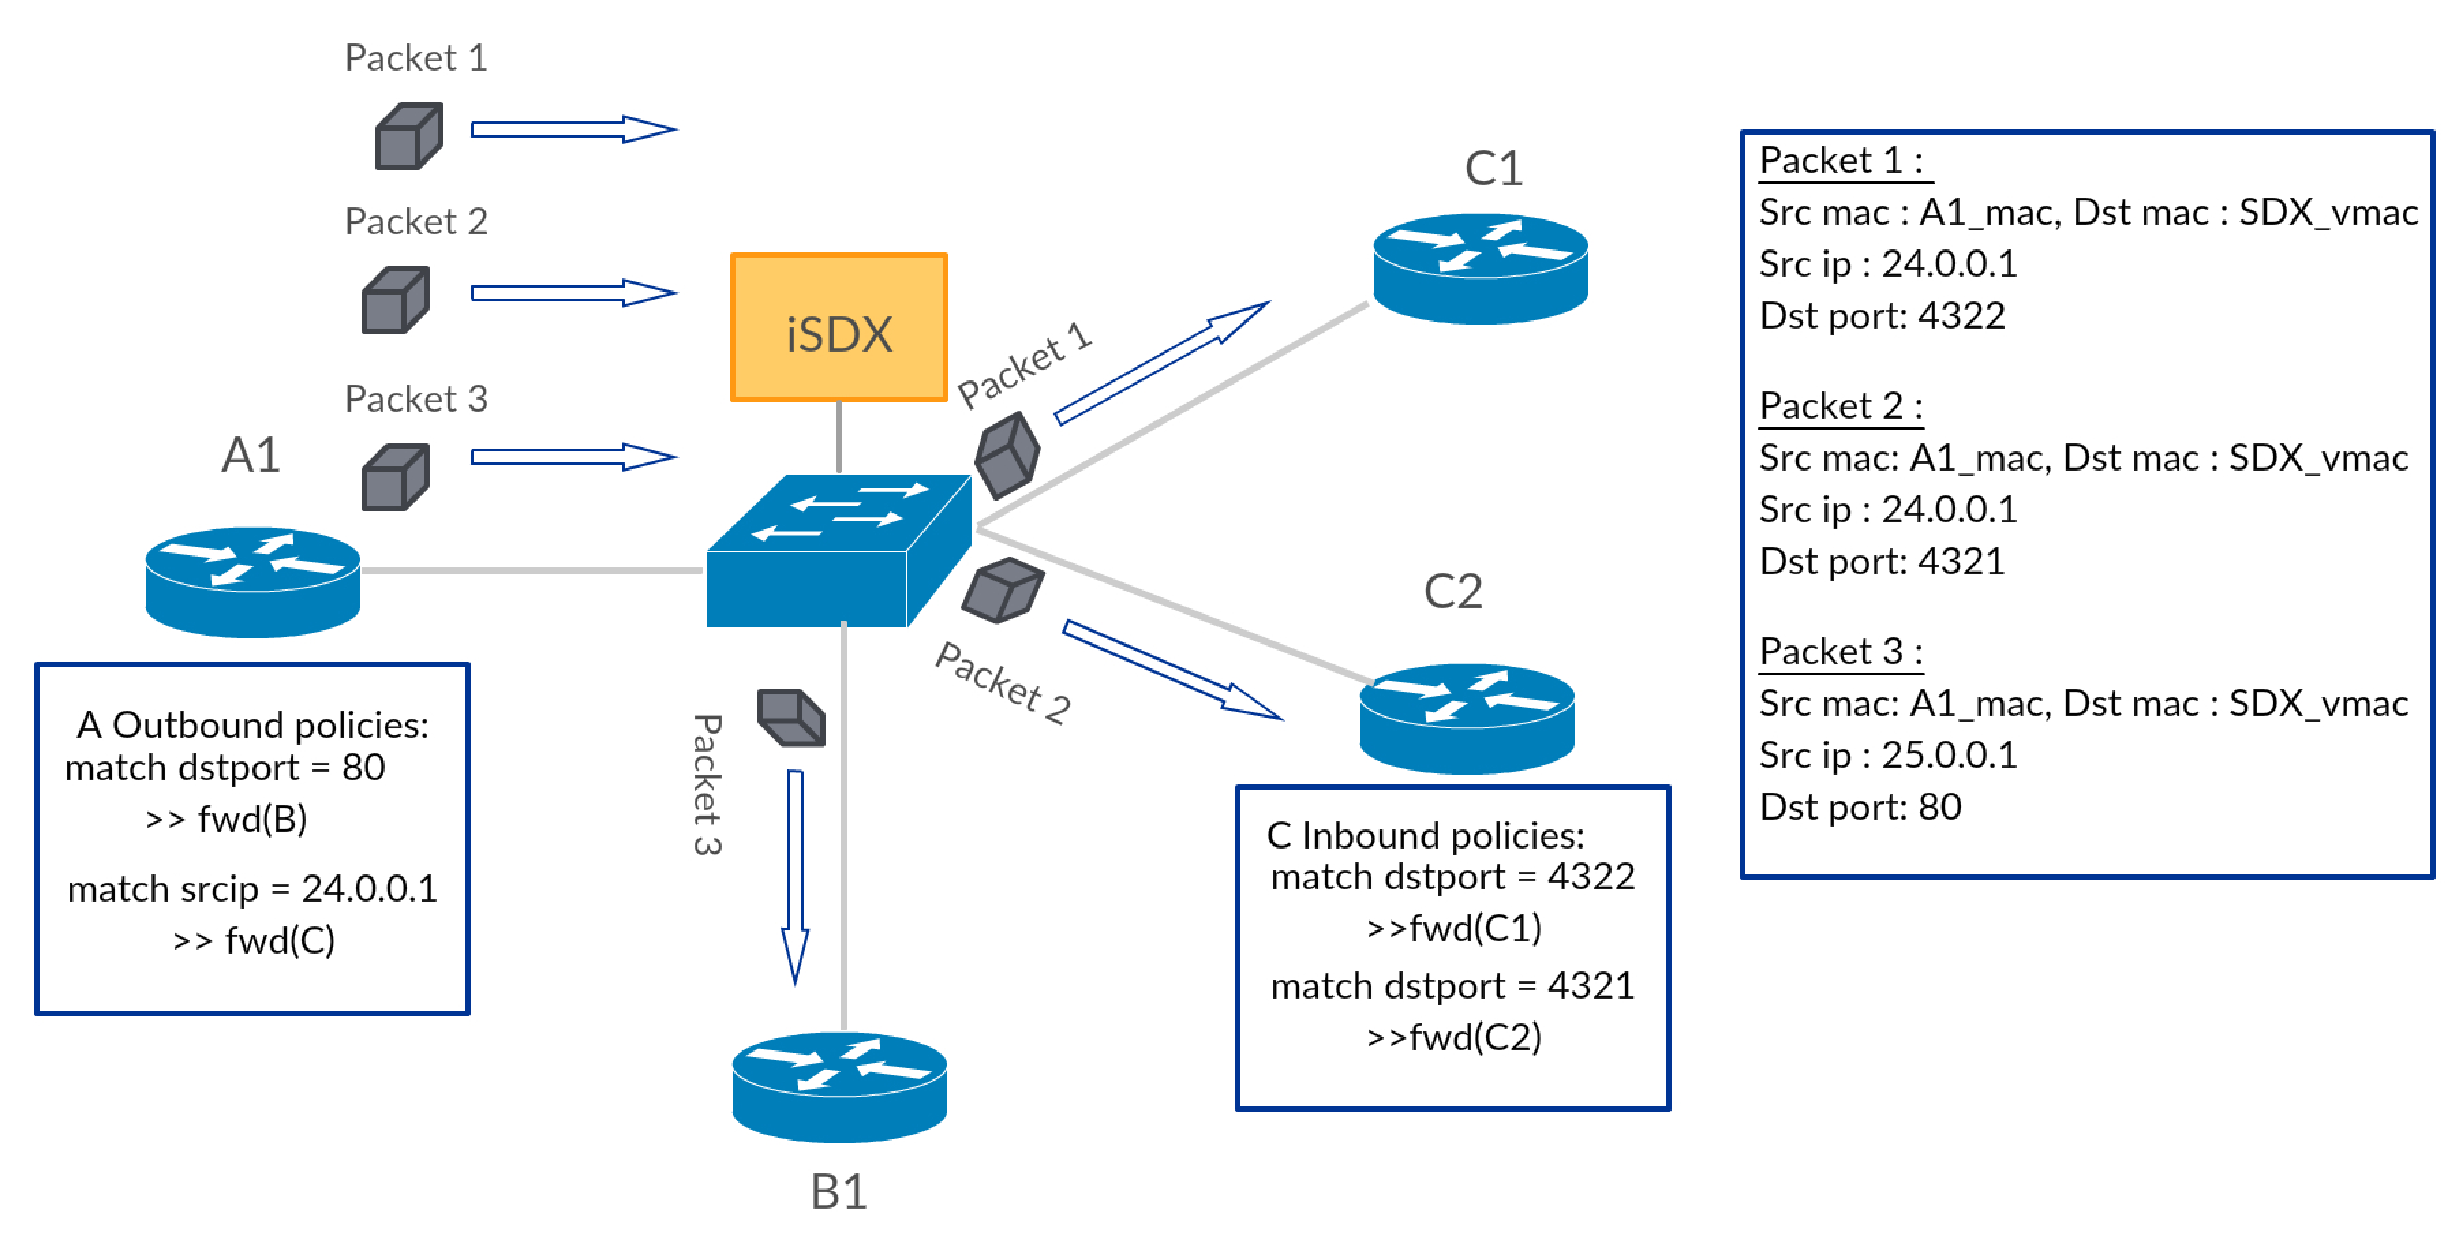
\includegraphics[scale = 0.32]{../Figures/bckgrnd_sdx_policies.pdf}
\caption{Example of outbound and inbound policies with an iSDX connected to three \\ participants}
\end{figure}


\subsection{\label{chapter2:iSDX:virtual next-hop, virtual mac address}virtual next-hop, virtual mac address}
In order to not violate BGP advertisements (send packets to participants that did not advertise the prefix of the packet) the iSDX uses the destination mac address as a data plane tag. \\ 
In the destination mac address the iSDX encodes the participants advertising the prefix of the packet and the BGP best next hop participant for this prefix. This mac address corresponds to a virtual next hop, which is assigned to every prefix. \\ The iSDX sends BGP updates to the participants, with the next-hop of the update set to the virtual next-hop of the prefix. The virtual mac address is communicated to the participants via ARP.
\paragraph{\label{chapter2:iSDX:virtual next-hop :inbound policies}iSDX vmac:}

\begin{tabular}{|r|l|}
  \hline 
  participants advertising the prefix & BGP best next-hop participant \\
  \hline
\end{tabular}

\begin{figure}[h]
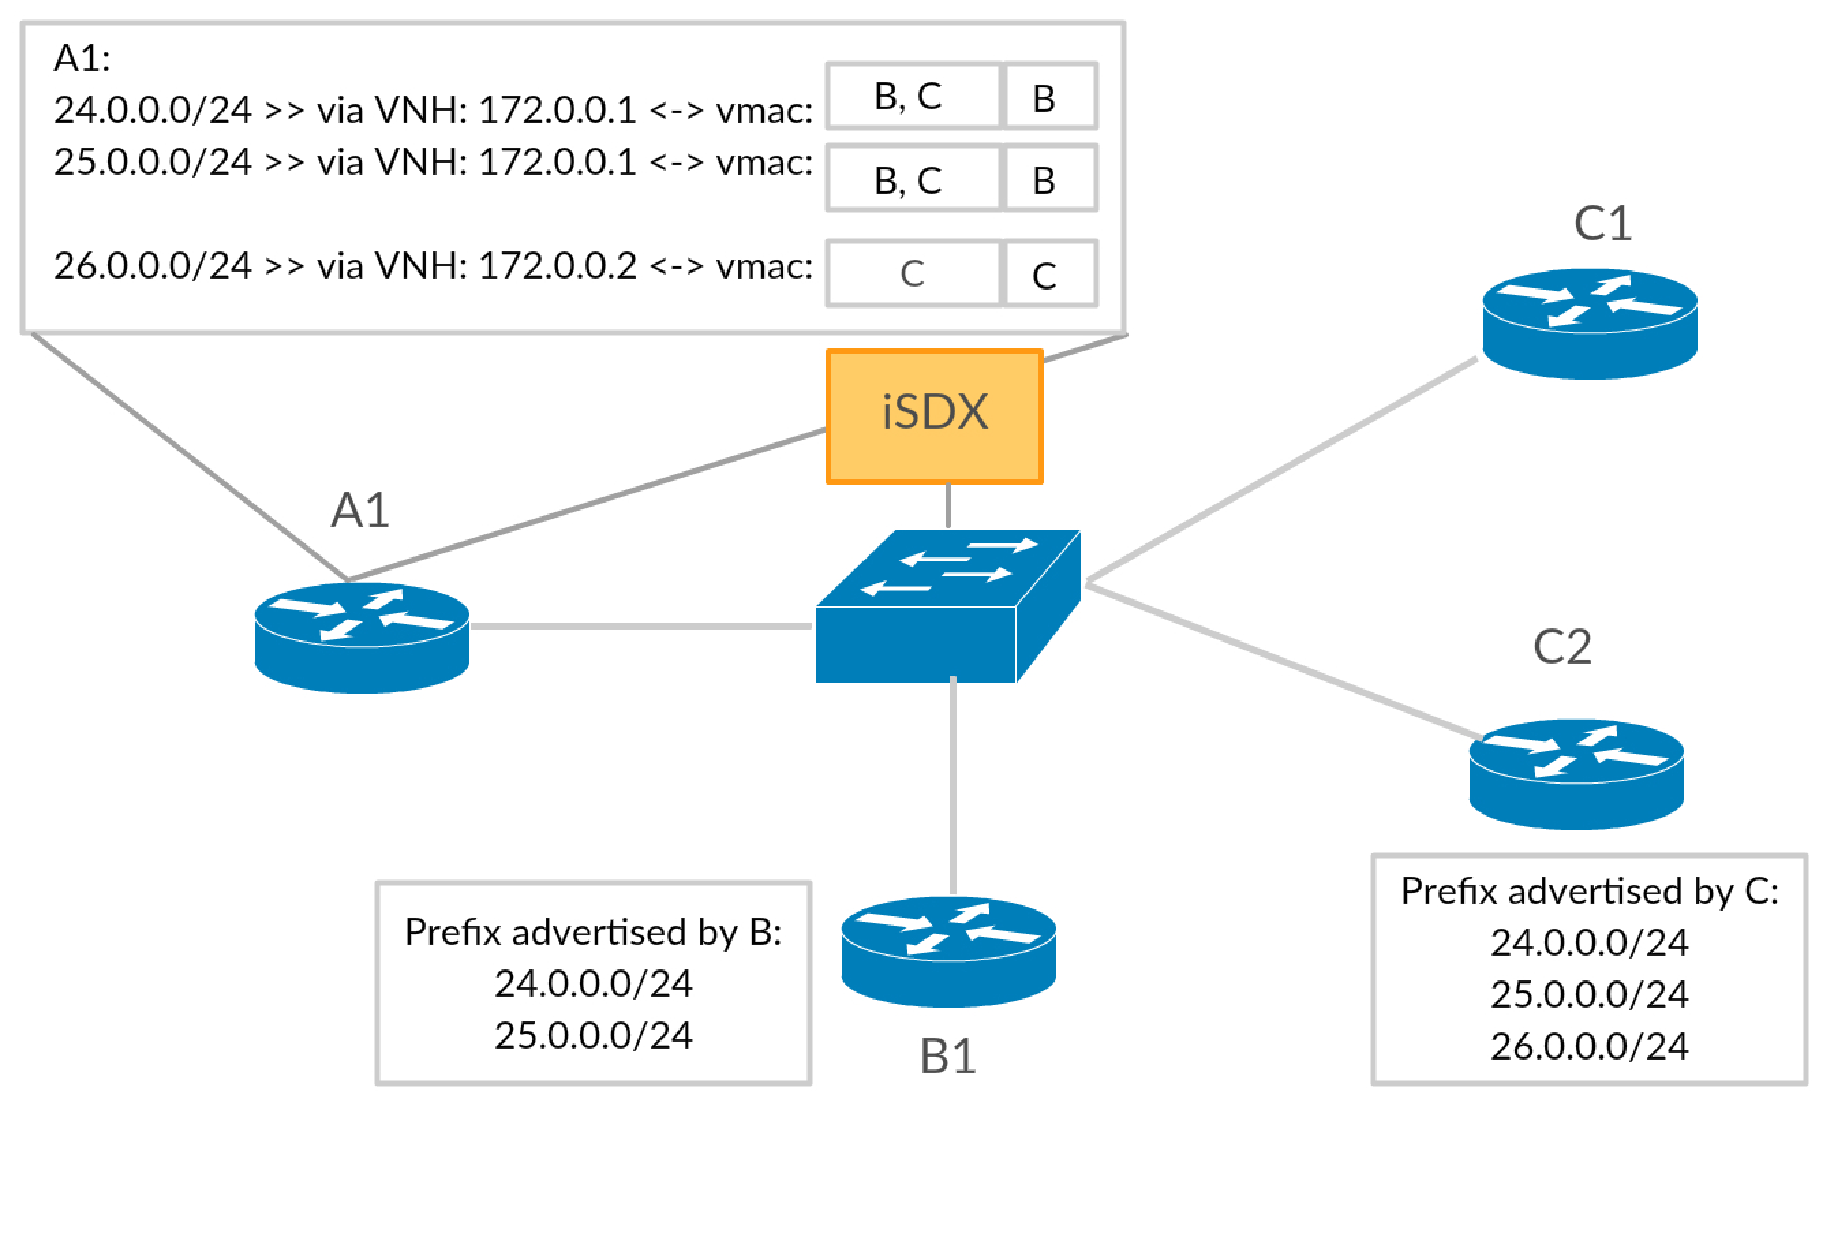
\includegraphics[scale = 0.36]{../Figures/intro_sdx_vmac.pdf}
\caption{Example of the iSDX vmac with an iSDX connected to three participants}
\end{figure}

\subsection{\label{chapter2:iSX:iSDX architecture}iSDX architecture}
\begin{figure}[h]
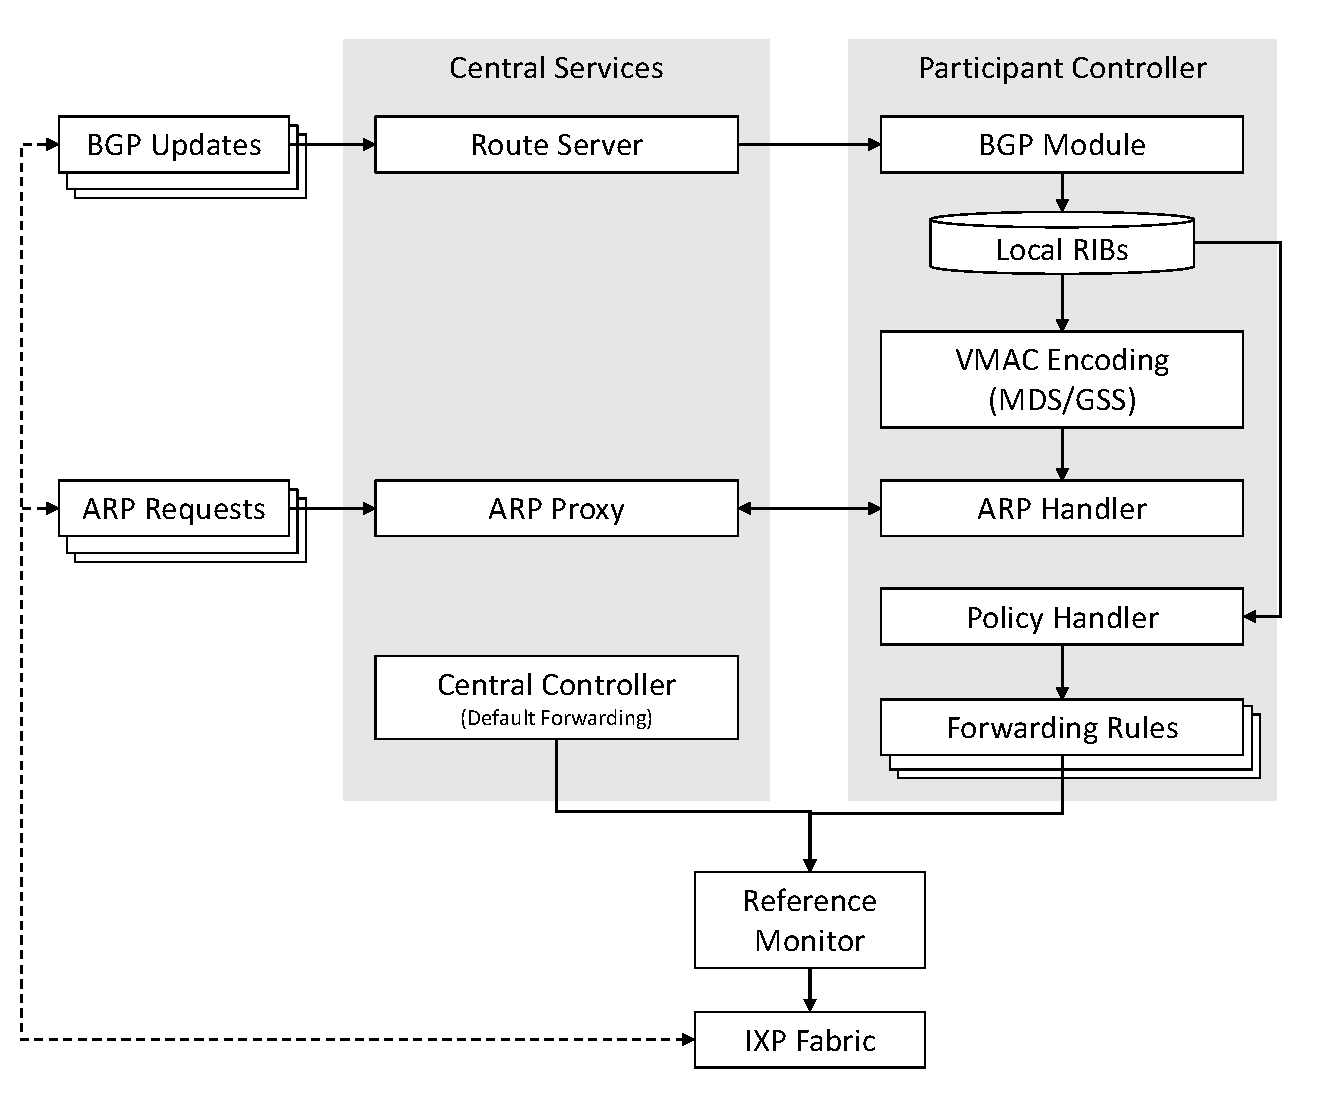
\includegraphics[scale = 0.4]{../Figures/bckdgrnd_sdx_architecture_cropped.pdf}
\caption{iSDX architecture}
\end{figure}

The iSDX architecture has two main Parts. The Central Services and the Participant Controller. Every participant has its own participant controller. \\
Central Services forwards BGP updates and ARP queries to the corresponding participant controller. It also initializes all the static flow rules. \\
The participant controller receives BGP updates from the Route Server. It then actualizes it's RIB checks if the virtual mac address was changed by the received BGP update, if so sends a gratuitous ARP to the ARP proxy. The participant controller also manages each participant's inbound and outbound policies. 

\section{\label{chapter2:Swift}Swift}

Swift is a prediction and fast-reroute framework to improve the convergence time of a BGP speaking router upon remote failure. Swifts prediction relies on the fact that the cause of a burst of withdrawals can be determined before receiving all the withdrawals. \\ Swift uses a SDN switch connected to the swifted router, it's neighbors and to the Swift controller. 


\begin{figure}[h]
\center
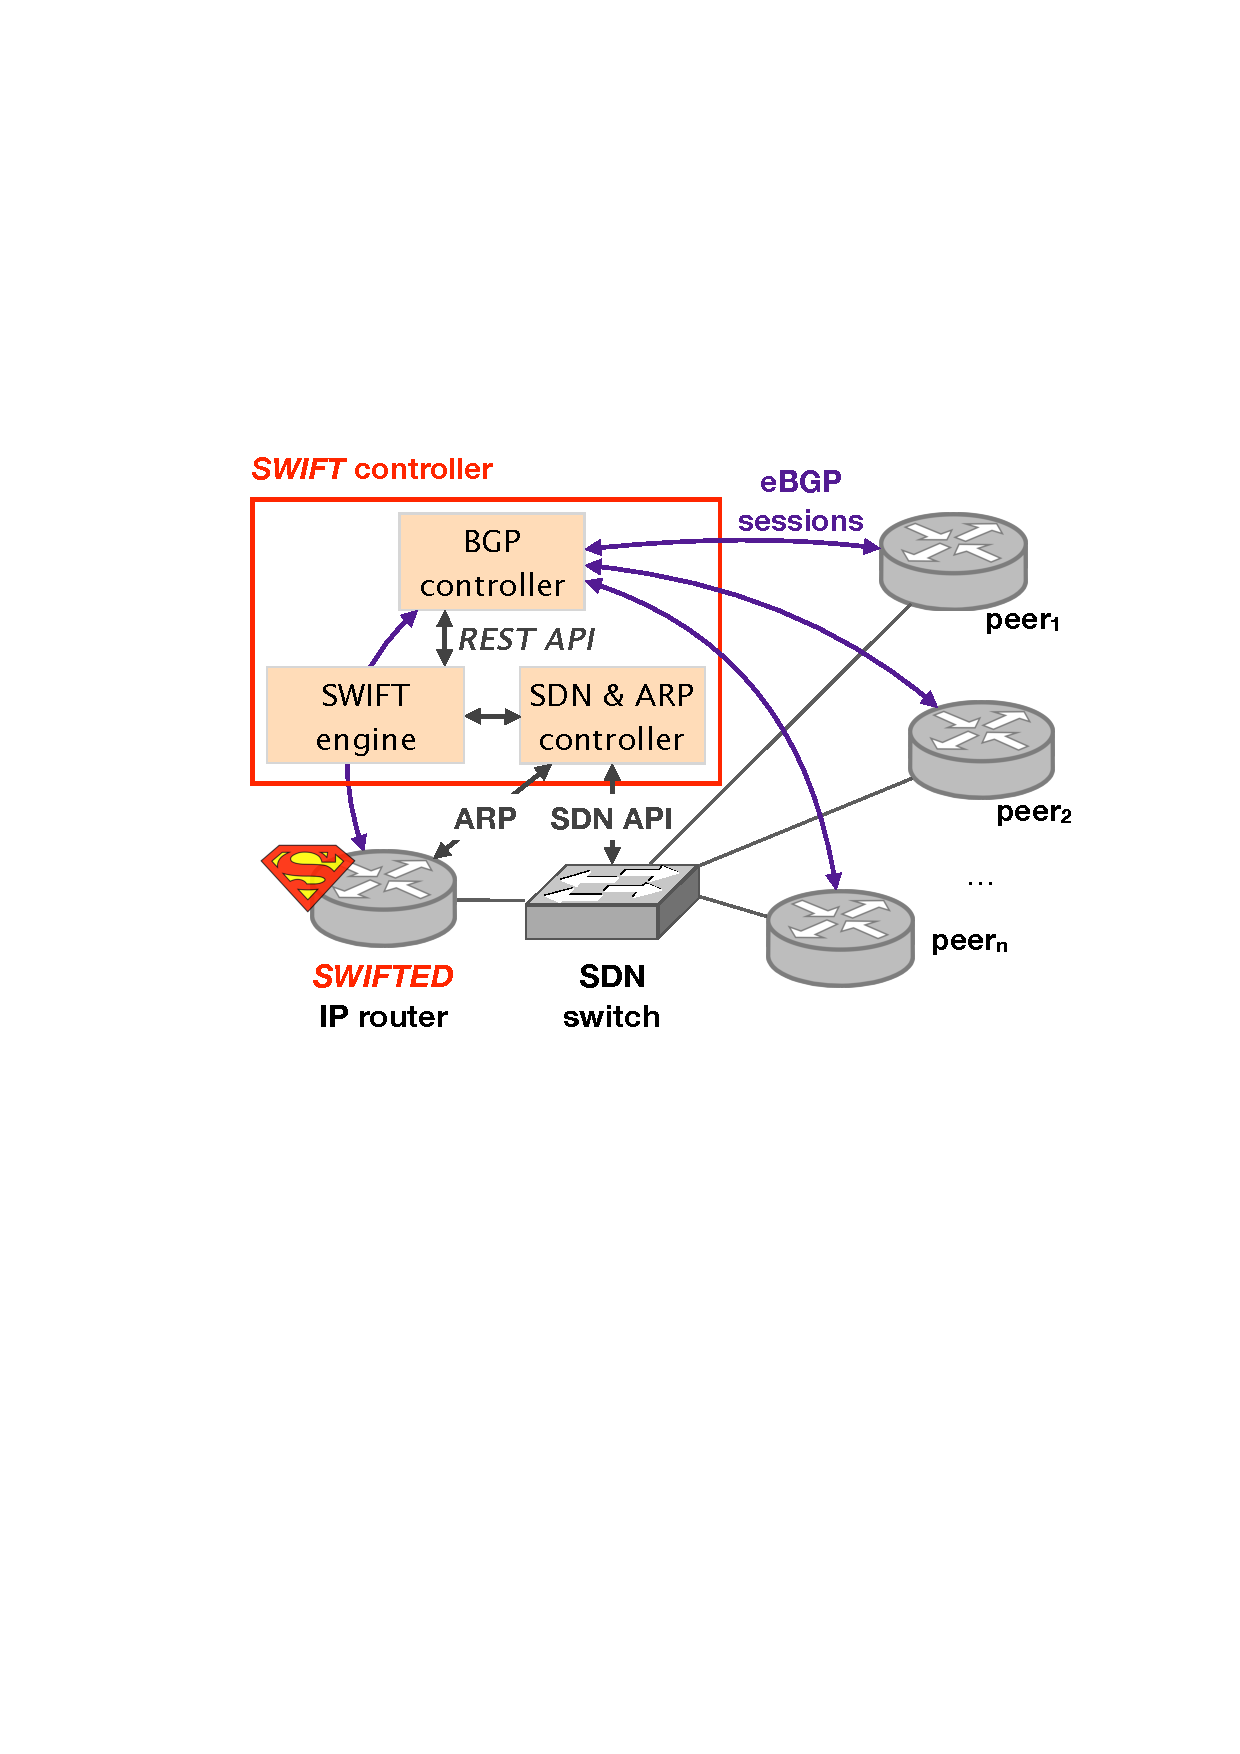
\includegraphics[scale = 0.5]{../Figures/bckgrnd_swift_architecture.pdf}
\caption{Example topology of a swifted router}
\end{figure}

The Swift Controller has two main modules: the burst prediction algorithm and the encoding of routing information. 

\subsection{\label{chapter2:Swift:encoding of routing information}encoding of routing information}
Swift similarly to the iSDX uses virtual next-hops and the destination mac address to encode information about the packet's prefix.\\
For every prefix Swift encodes the AS-path up to a certain depth and the backup next-hops for each AS-link on that AS-path. This encoding is then mapped to a virtual next-hop. When the swifted router wants to send a packet to any prefix it will use the virtual next-hop assigned by Swift. The virtual next-hop directly maps to the destination mac address. 

\paragraph{\label{chapter2:Swift:Swift vmac}Swift vmac:}

\begin{tabular}{|r|l|}
  \hline 
  backup next-hops for AS-links & AS-path \\
  \hline
\end{tabular}


\begin{figure}[h]
\center
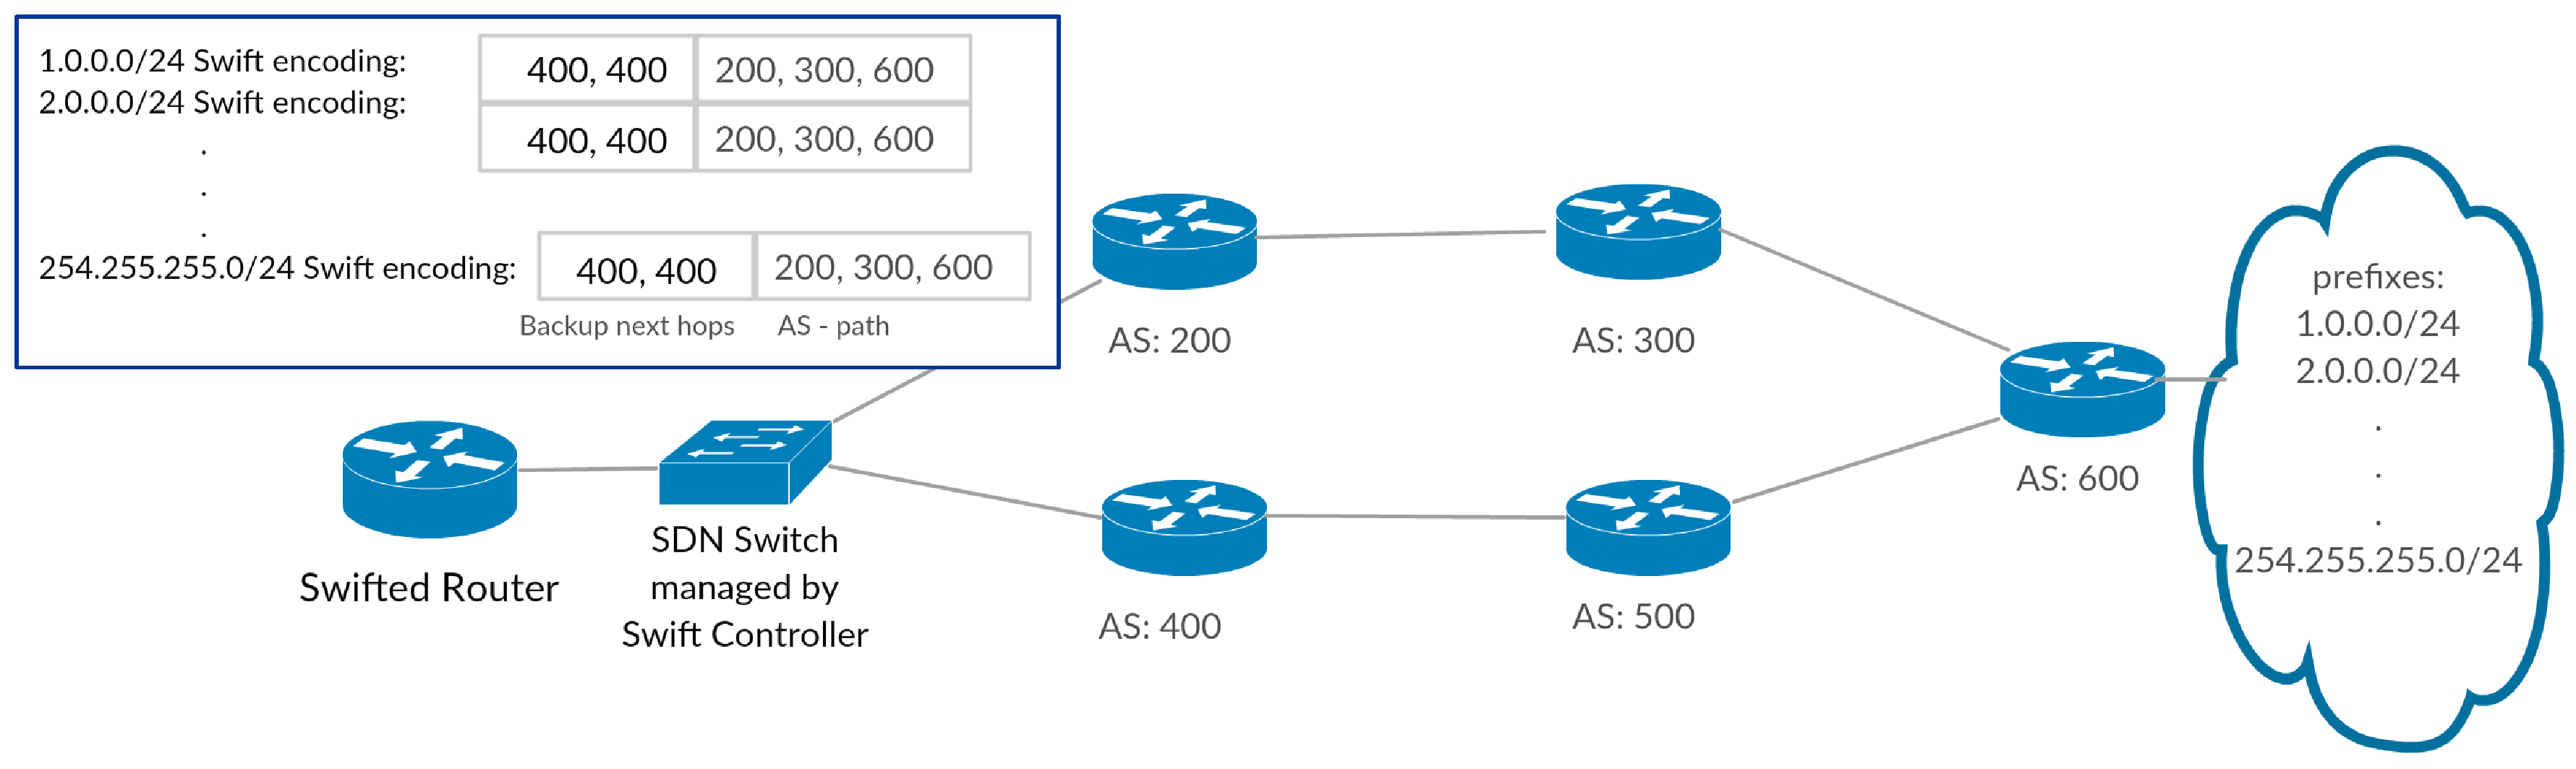
\includegraphics[scale = 0.24]{../Figures/bckgrnd_swift_topology.pdf}
\caption{Example of the Swift vmac}
\end{figure}


\subsection{\label{chapter2:Swift:burst prediciton algorithm}burst prediction algorithm}
The burst prediction algorithm takes BGP updates. It uses the updates to build a AS-topology. Once enough withdrawals arrive in a time frame short enough to trigger a burst, the burst prediction algorithm uses the withdrawals and the AS-topology to predict the failed AS-link. \\
Upon predicting a failed link the Swift Controller pushes flow rules int the SDN switch matching on the failed AS-link and on the corresponding backup next-hop. \\
Every packet that traverses the failed link (has the failed AS-link in it's AS-path encoding) will get rerouted to the backup neighbor.
\begin{figure}[h]
\center
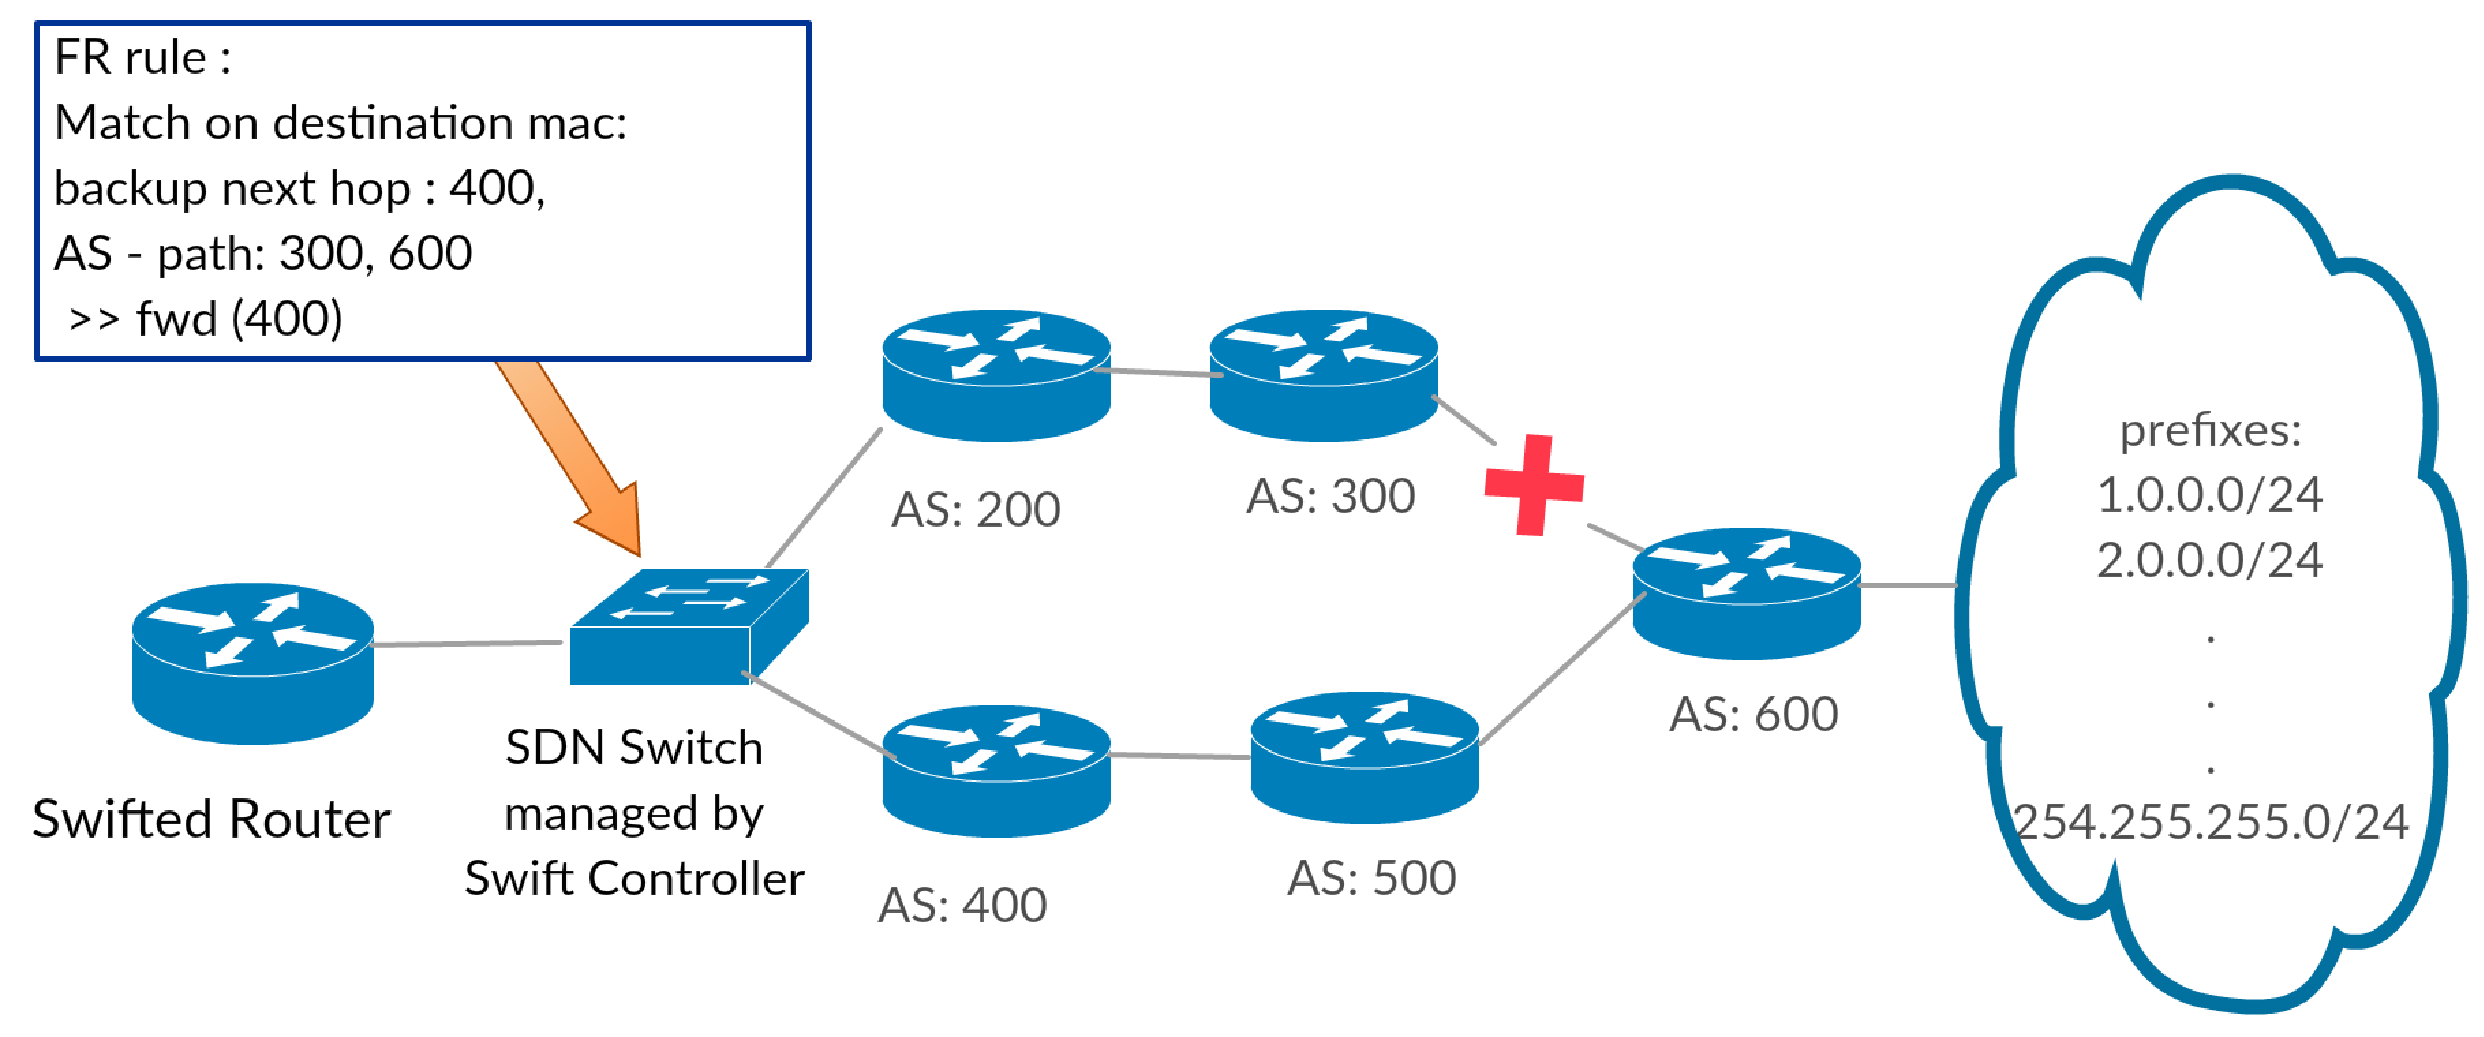
\includegraphics[scale = 0.36]{../Figures/bckgrnd_swift_fr.pdf}
\caption{Example of a fast-reroute after BPA predicts the AS link 300 600 to be down}
\end{figure}

By predicting the failed link and pushing fast-reroute rules instead of waiting for all withdrawals to arrive, Swift reduces the convergence time of the swifted router significantly.


\section{\label{chapter2:Motivation}Motivation}

The iSDX takes a long time to converge upon remote failure. The main problem is that the iSDX needs to do some additional computing a traditional BGP-router does not need to do. \\
When receiving a withdrawal the iSDX participant controller updates it's RIB, checks if the policy flow rules have changed and if the virtual next hop/vmac has changed. This additional computation adds a significant overhead to the convergence time of the iSDX. \\
Implementing Swift into the iSDX promises to significantly reduce the convergence time. Convergence time being the time until packets get sent to the correct participant and not into a black hole. \\
The main reason why implementing Swift in the iSDX is reasonable is their similar architecture. Both the iSDX and Swift use a SDN switch to program flow rules to steer traffic. They both are connected to BGP speaking routers and receive BGP updates from them. Swift and iSDX both use the destination mac address to encode information about a prefix and use the next-hop to map this vmac to a prefix. In addition the swift framework allows multiple swifted routers to be connected to the SDN switch, which in the iSDX's case means that all the participants will benefit from Swift.







%** Design.tex: How was the problem attacked, what was the design
%               the architecture 
\chapter{\label{chapter3}Implementation}

In this chapter, we show how Swift was implemented into iSDX. We give an overview of the modified iSDX architecture in \ref{chapter3:Architecture}. We explain the two new modules that were added to the iSDX in \ref{chapter3:Swift-BPA} and in \ref{chapter3:FR-handler}, respectively. We explain what was changed in the default iSDX modules in \ref{chapter3:Changes_to_the_iSDX} and explain the VMAC partitioning in \ref{chapter3:vmac_partitioning}.

In the next chapter we present the results of the tests done to measure the convergence 
performance of the iSDX.

\section{\label{chapter3:Architecture}Architecture}

\begin{figure}[h]
\center
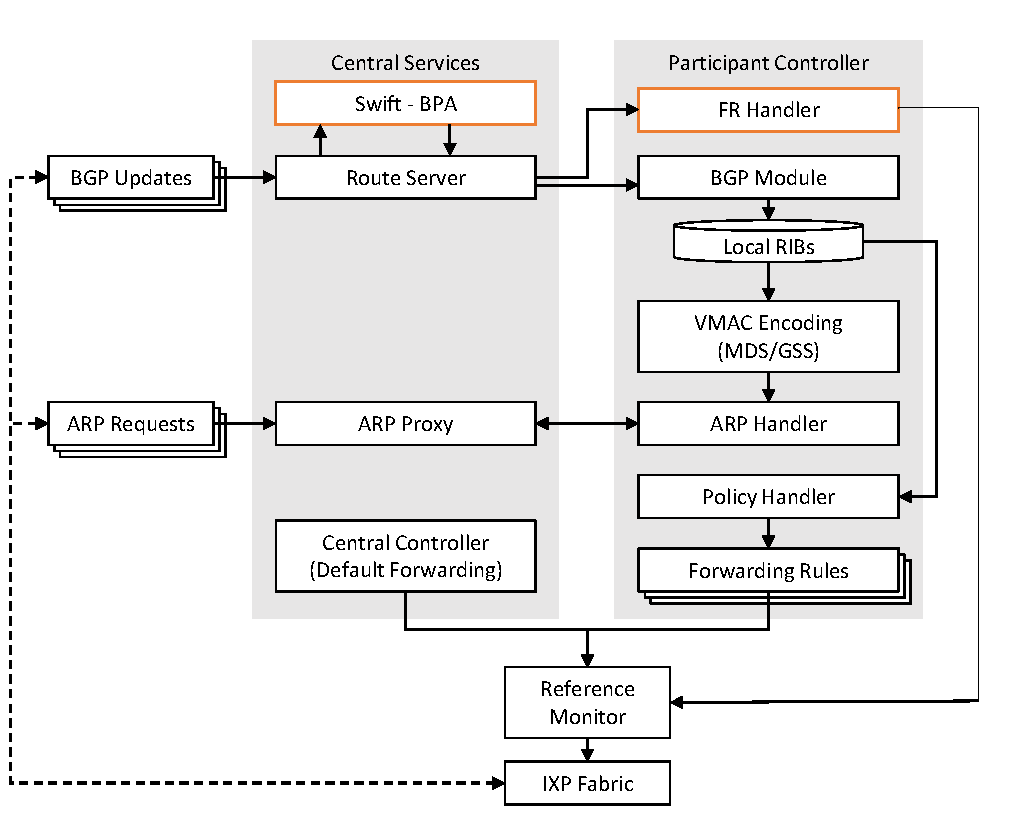
\includegraphics[scale = 0.7]{Figures/design_sdx_swift_cropped.pdf}
\caption{iSDX architecture with Swift}
\label{fig:isdx_architecture_with_swift}
\end{figure}

Figure~\ref{fig:isdx_architecture_with_swift} shows the iSDX~\cite{feamster2013sdx} architecture with Swift. The orange modules represent the new modules we had to add to the iSDX to implement Swift. The iSDX receives two additional modules the Swift-BPA module in the central services and the FR handler in the participant controller. With these two modules the iSDX will now detect bursts of withdrawals, predict the failed AS-link and push fast-reroute rules into the IXP fabric. \\
In the following sections, I will go over the functionality of the new modules and other changes to the iSDX in more detail.

\section{\label{chapter3:Swift-BPA}Swift-BPA}

\begin{figure}[h]
\center
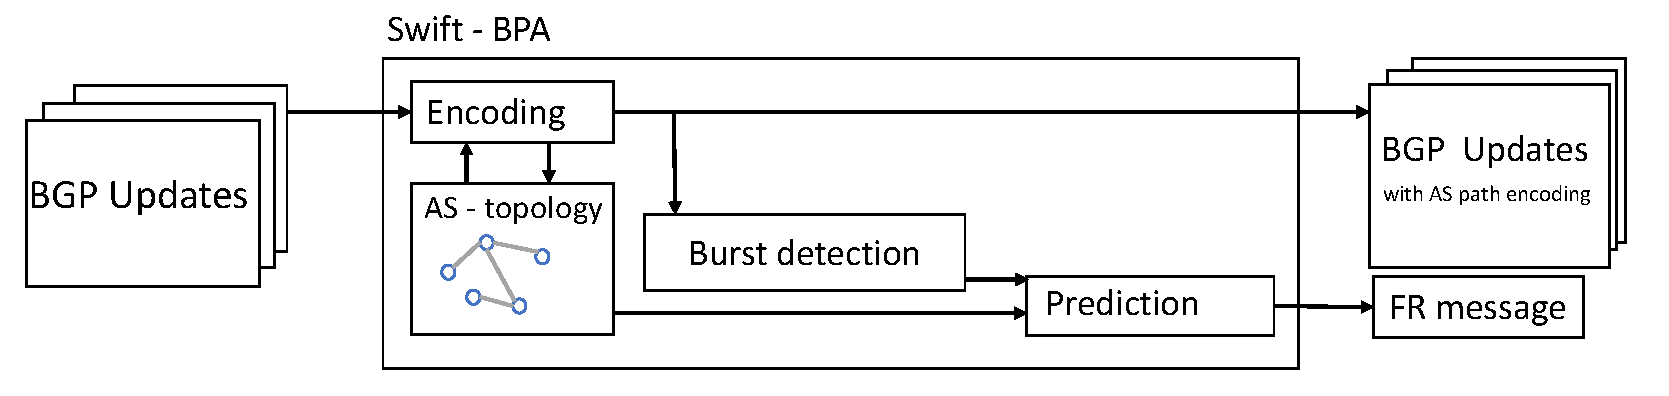
\includegraphics[scale = 0.5]{Figures/design_swift_bpa_cropped.pdf}
\caption{pipeline of the Swift-BPA module}
\end{figure}

The Swift-BPA module implements Swifts main functionality, encoding and prediction. It is part of the central services and exchanges BGP updates and FR messages with the route server.

\rb{write that the Swift-BPA module is placed at the route server and processes each update before passing it on to the participant controllers. I would not write that it receives the update from the route server and sends it back, but that it is part of the route server. Also, split the explanation in two parts: First, the encoding and the prediction. It handles all the updates, adds the encoding to it and sends it to the participant controllers. In parallel, it updates the AS-topology and keeps track whether a burst is triggered or not.}
The Swift-BPA module receives BGP updates from the route server. It then adds the AS-path encoding to the BGP update and sends the modified BGP update back to the route server.

The Swift-BPA then checks if the received BGP updates are enough to trigger a burst. If so it starts the prediction process. At the end of the prediction the Swift-BPA sends a fast-reroute message to the route server. The fast reroute message informs the participant controllers about the AS-link that is predicted to be down. The route server forwards the FR message to the participant controllers.

Similiar to the participant controller every participant has a Swift-BPA process running. The Swift-BPA only receives BGP updates from his own routers. This way the Swift engine can be implemented without any modifications.

\section{\label{chapter3:FR-handler}FR-Handler}

\begin{figure}[h]
\center
\includegraphics[scale = 0.6]{Figures/design_fr_handler_cropped.pdf}
\caption{pipeline of the fast reroute handler}
\end{figure}

The FR-handler implements the pushing of fast reroute rules.  \\
Once the Swift-BPA predicts a failed AS-link it sends FR messages to all the participant \\ controllers.
The FR-handler receives FR messages and computes the fast reroute rules using the backup next-hops and the predicted AS-link. Every participant controller computes its own backup next-hops. \\ The fast reroute rules get sent to the reference monitor as flow rule messages. The reference monitor then installs the flow rules in the SDN switch. Just like in Swift the fast reroute rules match on the failed AS-link and on the backup next-hop.    

\newpage

\section{\label{chapter3:Changes_to_the_iSDX}Changes to the iSDX}

We also had to apply a few changes to the iSDX's modules. These changes mainly affect the route server, the local RIB of the participant controller and the VMAC encoding. 

\paragraph{\label{chapter3:Changes to the iSDX:route server}Route Server:}

\rb{The route server had to adapted to work with the Swift-BPA module. etc.}

The route server now has two modules the Listener and Sender. \\
The Listener receives BGP updates and forwards them to the Swift-BPA. \\
The Sender receives modified BGP updates and FR messages from the Swift-BPA and forwards them to the participant controllers. The sender processes FR messages with higher priority than modified BGP updates, this way the FR messages reach the FR handlers as quickly as possible. 

\begin{figure}[h]
\center
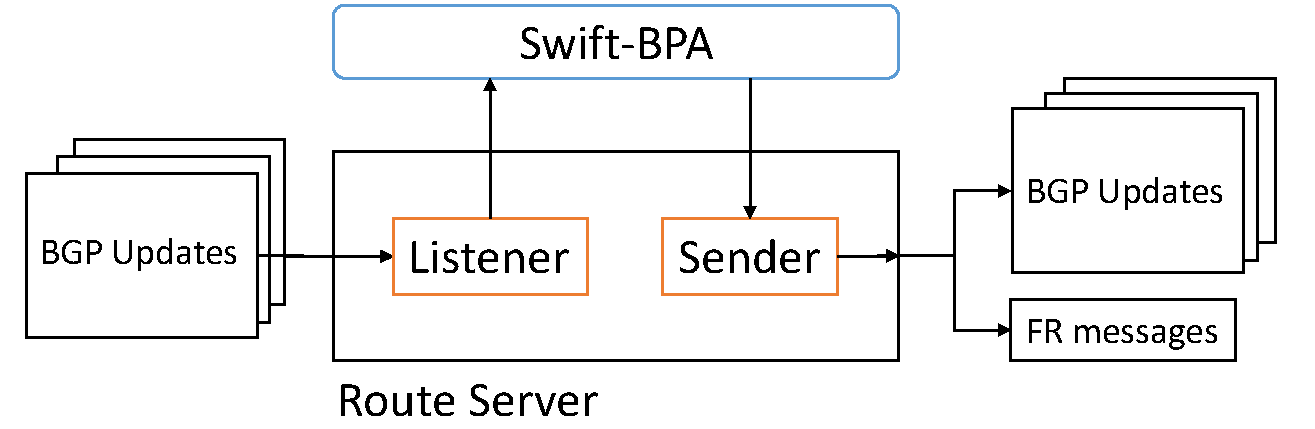
\includegraphics[scale = 0.45]{Figures/design_route_server_cropped2.pdf}
\caption{pipeline of the modified route server}
\end{figure}


\paragraph{\label{chapter3:Changes to the iSDX:local RIB}Local RIB:}
\rb{extend it a bit.}
The local RIB now stores the AS-path encoding. The AS-path encoding is then used in the VMAC encoding. 

\paragraph{\label{chapter3:Changes to the iSDX:Vmac Encoding}VMAC Encoding:}
The VMAC encoding now computes the backup next-hops for the AS-path of the BGP update. There is one backup next-hop for every AS-link on the AS-path, packets can be sent to the backup next-hop in case this AS-link is predicted to be down. \\
The VMAC encoding now builds the VMAC using both iSDX and Swift encoding. \\
\rb{better switch the order} More in section \ref{chapter3:vmac_partitioning} 

\section{\label{chapter3:vmac_partitioning}VMAC Partitioning}

Both Swift and iSDX use the destination mac address as a VMAC to encode additional information into the packet. \rb{it is not easy to use another field in the header for this purpose due to the provisiong with BGP next hop, ARP etc. Therefore, the destination has to be shared between iSDX and Swift.} The VMAC has to be shared between the iSDX and the Swift encoding. This is because the iSDX and Swift encode different information about the prefix. The iSDX encodes the participants advertising the prefix and the BGP best next-hop. Swift encodes the AS-path and the backup next-hops for each link on the AS-path.

The encoded AS-path starts with the second AS on the AS-path. This is because the first AS is already encoded as the BGP best next-hop. (in the iSDX part of the VMAC)

\begin{figure}[h]
\center
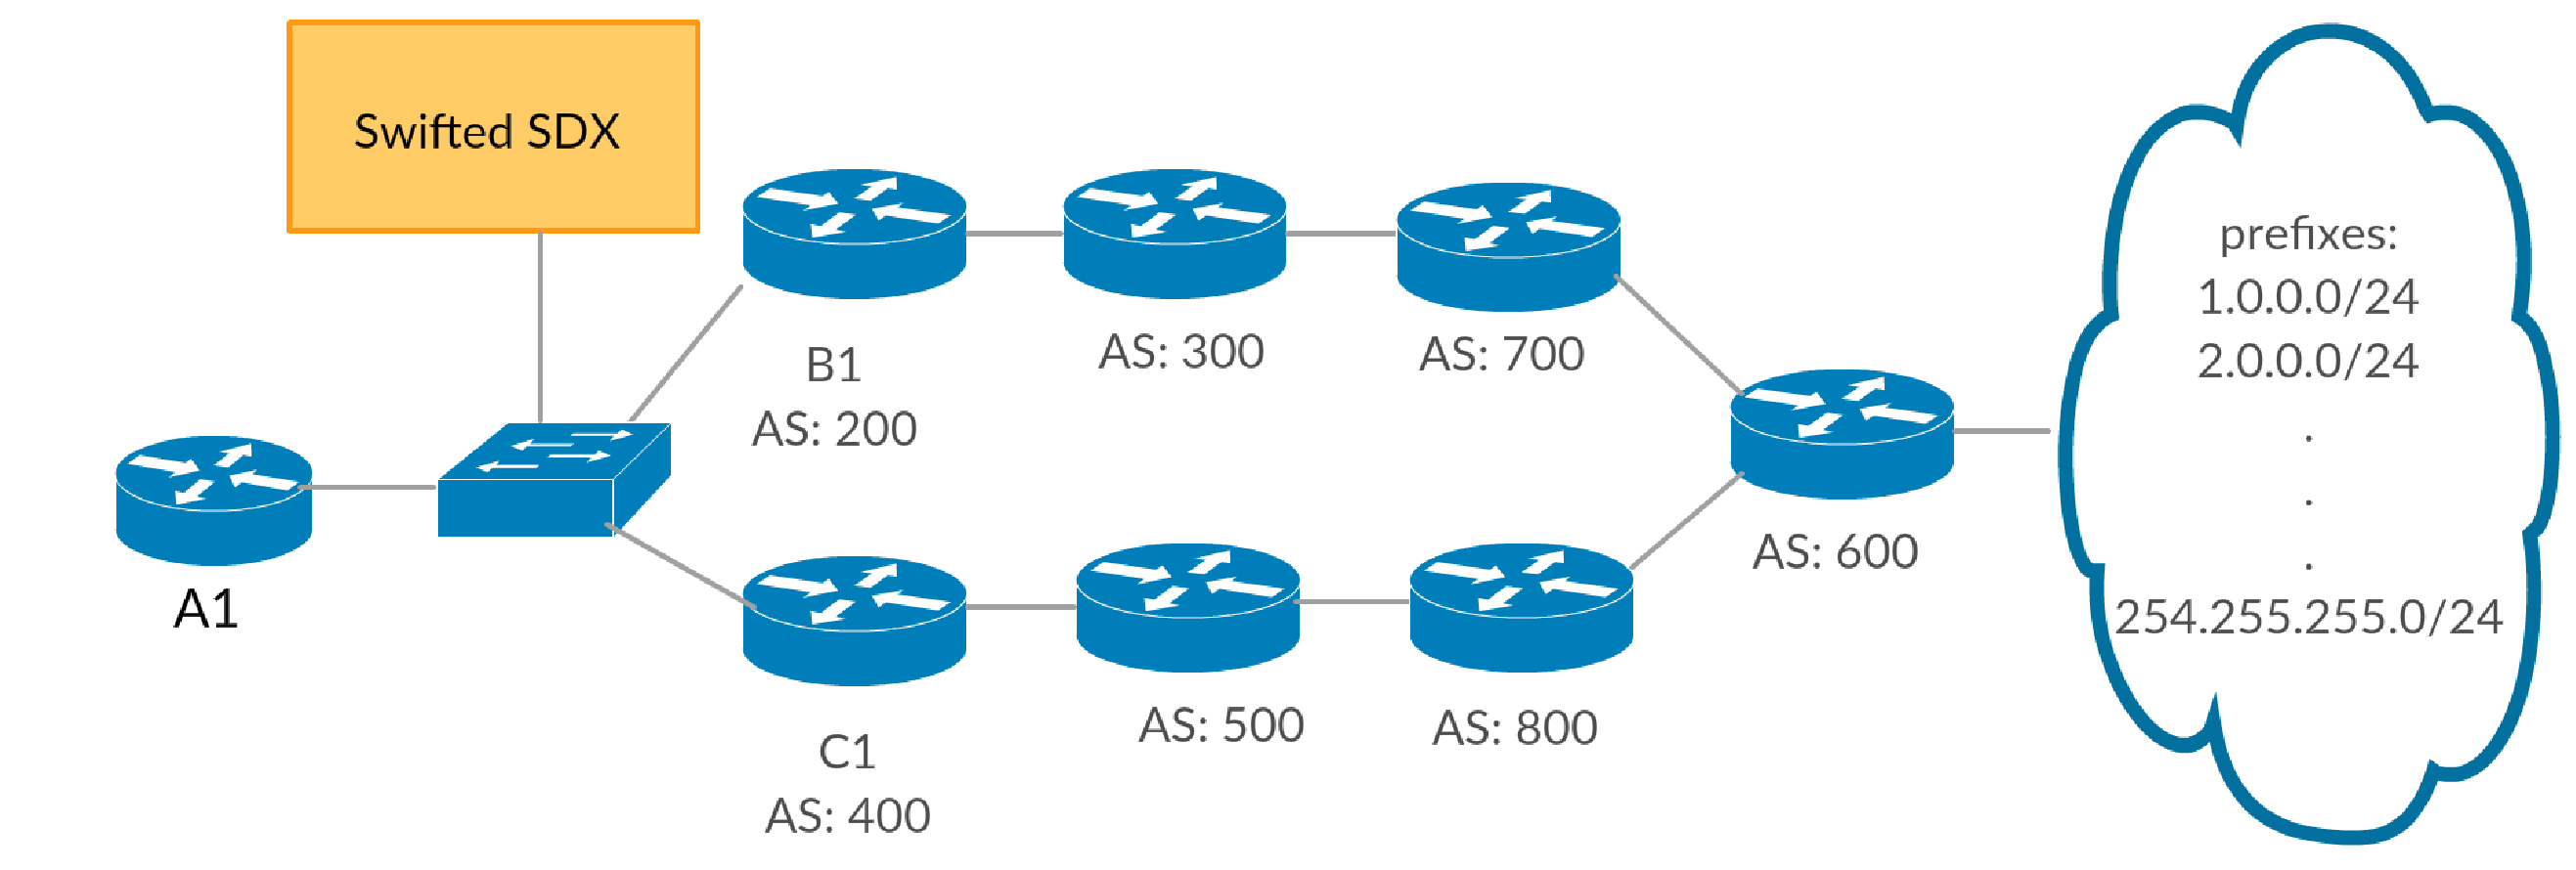
\includegraphics[scale = 0.24]{Figures/design_vmac_topology.pdf}
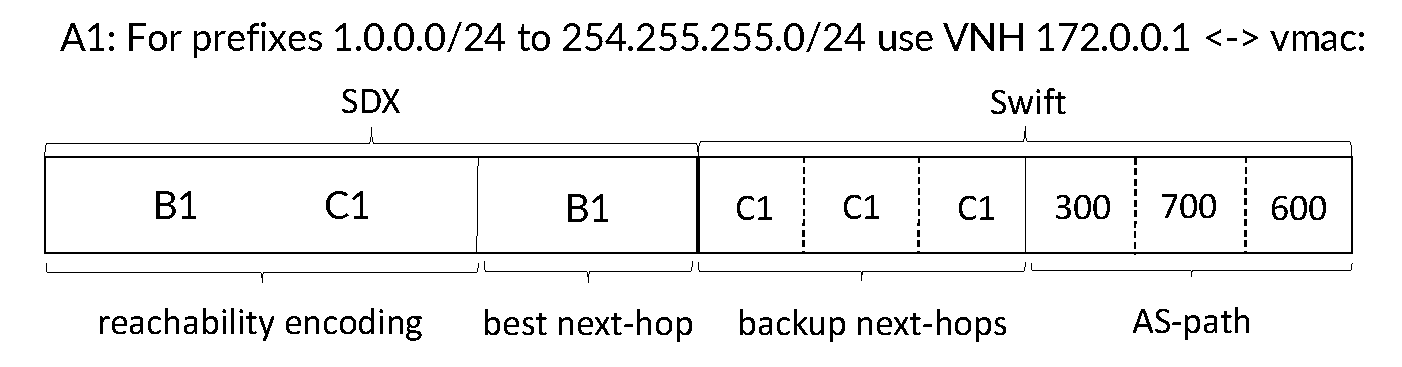
\includegraphics[scale = 0.35]{Figures/design_vmac_cropped.pdf}
\caption{example of the vmac in the iSDX with Swift}
\end{figure}

\newpage


%** Results.tex: What were the results achieved including an evaluation
%
\chapter{\label{chapter 4}Evaluation}

In this chapter I will evaluate the convergence time of the iSDX without and with Swift.
I will then examine the vmac partitioning and the number of flow rules required for a fast reroute.

\section{\label{chapter4:Test Setup}Test Setup}

\begin{figure}[h]
\center
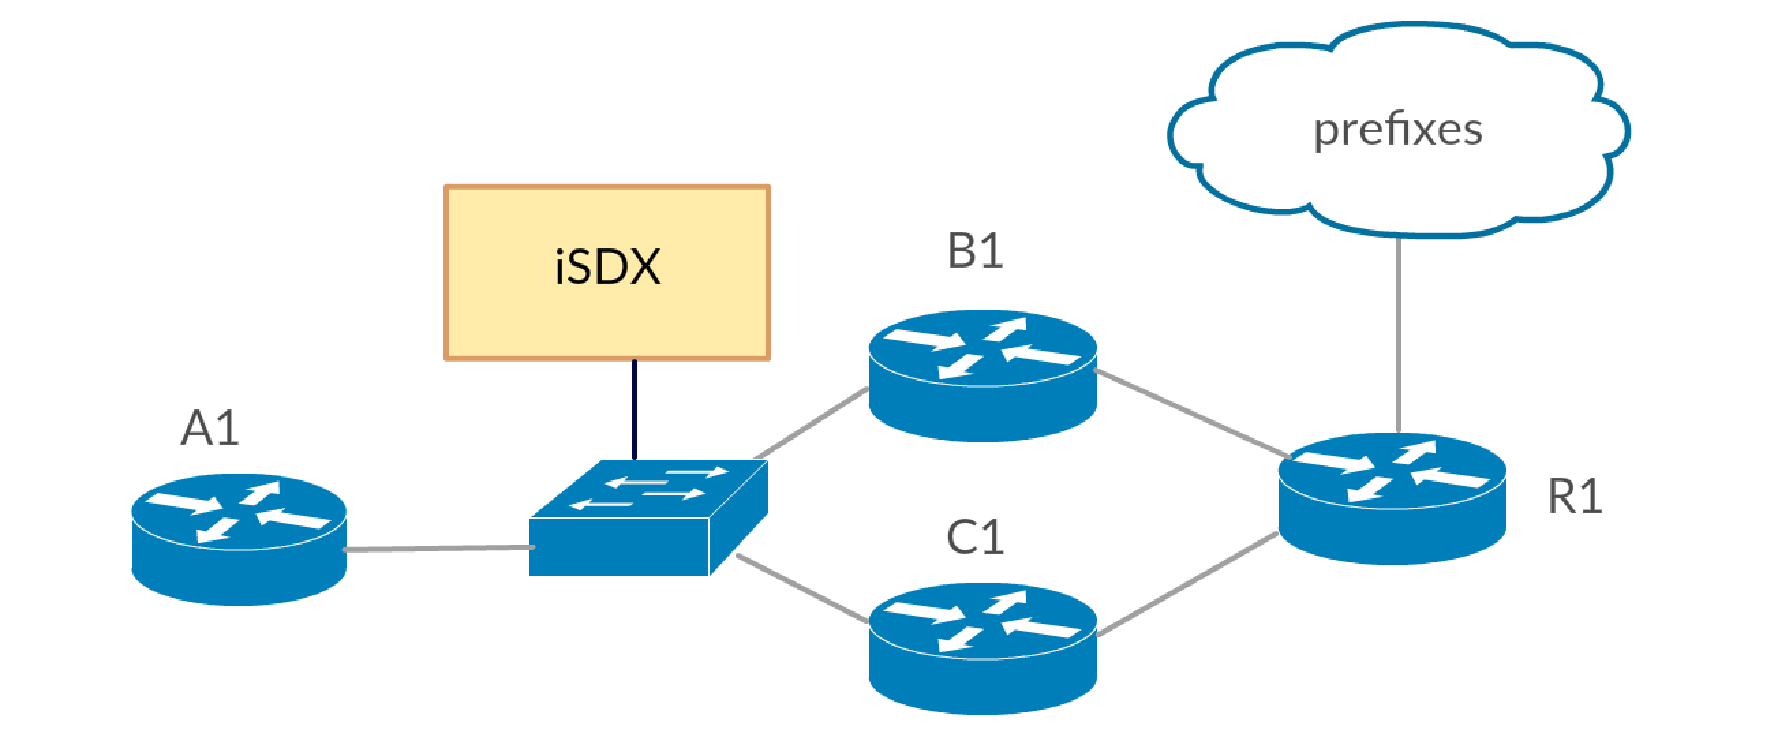
\includegraphics[scale = 0.36]{../Figures/eval_exp_setup.pdf}
\caption{Experiment Setup}
\end{figure}

The test setup has an iSDX with or without Swift connected to three participants. Participants B1 and C1 are connected to the rest of the internet via R1 and advertise up to 500000 prefixes to A1. Participant A1 prefers routes from B1. Remote failure is simulated by setting the link B1 R1 down. If this link is down A1 needs to updates his RIB, check if flow rules have changed and update the virtual next-hop/vmac for every withdrawn prefix.\\ 
The experiment setup is run in mininet. 



\section{\label{chapter4:Convergence time without Swift}Convergence time without Swift}

Convergence time is measured as the time between the first withdraw arriving in the route server and the participant controller finishing to process the last withdraw. To measure the convergence time the built in iSDX log server is used.\\
This convergence time does not take into account the hold timer or the time the participant router takes to process the withdrawals. But since these things are not under the control of the iSDX they are ignored in this evaluation.

\begin{figure}[h]
\center
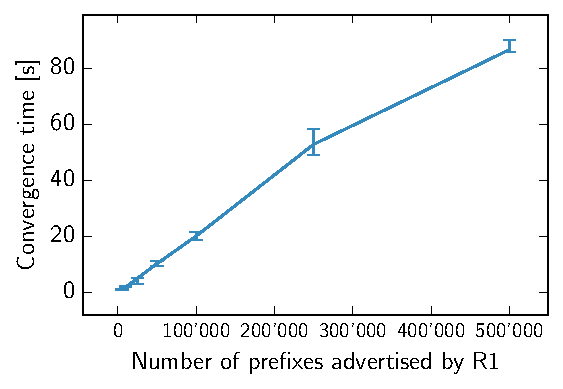
\includegraphics[scale = 1]{../Figures/noswift.pdf}
\caption{Convergence time of the iSDX without Swift}
\end{figure}

\newpage

The convergence time increases linearly with the number of prefixes advertised by R1. \\
At 500'000 prefixes the iSDX takes about 90 seconds to converge. During these 90 seconds A1 sends packet to B1, which then get dropped by B1. 

\section{\label{chapter4:Convergence time with Swift}Convergence time with Swift}

Convergence time is measured as the time between the first withdraw arriving in the route server and the participant controllers FR handler finishing to push the Fast-reroute rules. \\

\begin{figure}[h]
\center
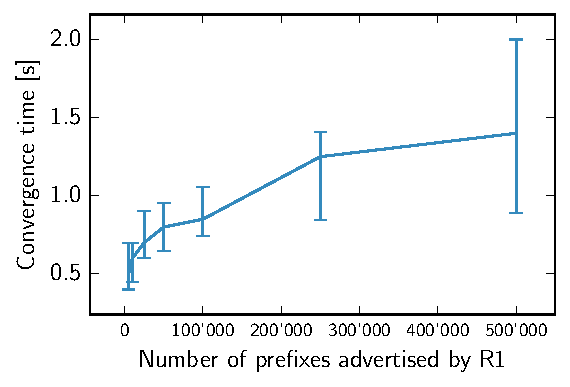
\includegraphics[scale = 1]{../Figures/swift.pdf}
\caption{Convergence time of the iSDX without Swift}
\end{figure}

The convergence time increases slightly with higher number of prefixes. At 500'000 prefixes the iSDX takes about 1.5 seconds to push the FR rules. After these 1.5 seconds packets sent from A1 get redirected to C1 and reach their destination. \\
For 500'000 prefixes the convergence time is reduced by a factor of 60.


\newpage

\section{\label{chapter4:vmac evaluation}vmac evaluation}

Since both the iSDX and Swift use the destination mac address to encode different information, the amount of bits available to  the iSDX and Swift is reduced. In this section the vmac partitioning in its current state will be analyzed.

\begin{figure}[h]
\center
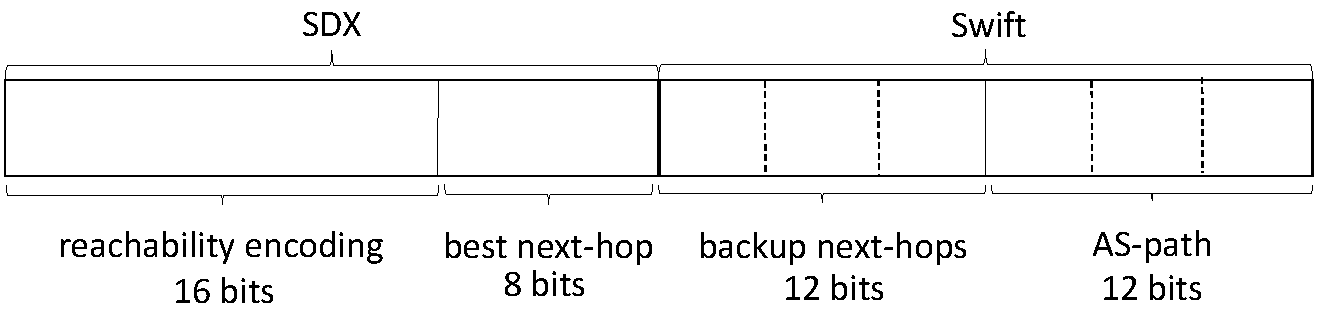
\includegraphics[scale = 0.65]{../Figures/eval_vmac_cropped2.pdf}
\caption{Vmac of the iSDX with Swift}
\end{figure}

In its current state 24 bits are allocated to the iSDX. 16 bits for the reachability encoding and 8 bits for the BGP best next-hop. \\
The amount of bits allocated for the best next-hop limits the number of participants the iSDX with Swift can have. The number of participants is limited to $2^8$ = 256. \\
24 bits are allocated to Swift. 12 bits are used to encode backup next-hops and 12 bits are used for the AS-path encoding. \\
With 12 bits used for the AS-path encoding the encoding has a coverage performance of about 85\%. (see Swift paper Figure 9)\\
12 bits for 3 backup next-hops means 4 bits for each next-hop. This means that every participant can have 16 backup next-hops at most. This is not a lot and after 16 backup next-hops have been assigned some prefixes will end up with no backup next-hop. On the other hand it also limits the number of fast reroute rules. 


\section{\label{chapter4:number of flow rules}number of flow rules}

After a fast reroute message has been received the FR handler pushes reroute rules into the IXP fabric. For every backup next-hop that the participant has stored a rule is pushed. This means the maximum number of rules pushed by a participant after a fast reroute is 16. \\
FR messages get sent to every participant so the maximum number of flow rules for all the participants is 256*16 = 4096. This amount of flow rules is not substantial enough to have a significant impact on the iSDX. With the number of participants limited to 256 and participants having a reasonbale number policies, the flow rule limit for current SDN switches should not be reached. (iSDX paper figure 3 (a) amsix paper figure 9 )\\


%** Outlook.tex: What needs to be done further, what is planed
%
\chapter{\label{chapter7}Conclusion}
In this project Swift was implemented in the iSDX without significantly changing either the iSDX or Swift.

The convergence time upon remote failure of the iSDX was significantly reduced without \\requiring a lot of additional flow rules. Swift adds a small overhead to the processing of a BGP update. 

Their similar architecture makes integrating one into the other intuitive but it also severely constrains the iSDX's ability to scale with a higher number of participants. This is due to the\\bottleneck created by the limited size of the destination MAC address. With the current design up to $256$ participants can be supported. At the time of writing, only $1.8\%$ of all IXPs have more than $256$ participants. \cite{ixps} 


If the iSDX with Swift should be deployed at an IXP with more participants, more bits need to be allocated to the iSDX part of the VMAC. This in turn impacts the performance of Swift, leading to traffic being unnecessarily redirected or failed links not being correctly detected. One might look into implementing a more lightweight fast reroute framework that does not need to encode information on the destination MAC address. 

Future work may include finding a optimal partitioning of the VMAC, enabling the participant controller to use more backup next hops and solving the conflict between outbound policies and FR rules

%** Summary.tex: What have you achieved, what have you presented in this
%                document.  What are the highlights of your work.
%                It should conclude by a conclusion.
%\chapter{\label{summary}Title}
Sum up what you have done and recapitulate your key findings.



%** Switch to appendix-mode in Latex.
%
\appendix

%** I would like to have the appendices enumerated by Alphabetical
%   characters.
\renewcommand{\thepart}{\Alph{part}}

%** appendix.tex: Install instructions, configurations, test results,
%		simulation data, additional theoretical disquisitions, ...
%
%%****************************************************************************
%** Copyright 2005 by Bernhard Tellenbach, <bernhard.tellenbach@airmail.ch>
%** Information is provided under the terms of the
%** GNU Free Documentation License <http://www.gnu.org/copyleft/fdl.html>
%****************************************************************************
%****************************************************************************
%** Last Modification: 2005-07-11 1600
%** 2005-07-11	Updated the syntax to match the current nomencl packet
%****************************************************************************

\chapter{\label{appendixA}Title}


\section{\label{chapterA:section1}Section 1}

\begin{verbatim}
All is presented exactely the way you write it.

Page boundaries are not checked.....................................................................................

\end{verbatim}

\chapter{\label{appendixB}Title}


%Entries for the list of abbrevations:
%
%To generate the list of abbrevations, execute:
%makeindex Thesis.nlo -s nomencl.ist -o Thesis.nls
%
%If you are using TeXniCenter, specify:
%"%bm.nlo" -s nomencl.ist -o "%bm.nls"
%as beeing the argument list for makeindex.
%---------------------------------------------------------------------------------------------------------
%For old nomencl package uncomment this:
%\printglossary
%For new nomencl package uncomment this:
\printnomenclature

\abbrev{XCA}{\markup{X}tremely \markup{C}ool \markup{A}bbrevations}




%** Timetable.tex: Timetable you worked out.
%
\chapter{\label{timetable}Title}
Here may come your thesis schedule (the original plan and ev. the actual outcome).

%** Originalproblem.tex: The problem statement you received.
%
\chapter{\label{originalproblem}Title}
Here comes the original task description that you agreed on with your supervisor/tutor.


%** bibtex is used to automatically generate the bibliography
%   references are stored in refs/refs.bib
%   use a bibliography manager like JabRef (http://jabref.sourceforge.net/) to manage refs/refs.bib
\bibliographystyle{abbrv}
\bibliography{refs/refs}

%** end the document environment
\end{document}
